% Claudia Porto, COMPLETE

The \textbf{Maximum Flow Problem} is a classical optimization problem in network theory, where the objective is to determine the greatest amount of flow that can be sent from a source vertex \( s \) to a sink vertex \( t \) in a directed graph \( G = (V, E) \), known as a flow network. Each edge \( (u, v) \in E \) in the network has a non-negative capacity \( c(u, v) \), representing the maximum allowable flow through that edge. The problem is subject to two fundamental constraints:
\begin{enumerate}
    \item Capacity constraint: The flow \( f(u, v) \) on any edge \( (u, v) \) must satisfy
   \[
   0 \leq f(u, v) \leq c(u, v),
   \]
   ensuring that the flow does not exceed the edge's capacity.
   \item Flow conservation constraint: For every vertex \( v \in V \setminus \{s, t\} \), the total flow entering \( v \) must equal the total flow exiting \( v \). Formally,
   \[
   \sum_{u \in V} f(u, v) = \sum_{w \in V} f(v, w),
   \]
   where \( f(u, v) \) denotes the flow from \( u \) to \( v \).
\end{enumerate}

\noindent At the source vertex \( s \), only outgoing flow is permitted:
\[
\sum_{v \in V} f(s, v) > 0,
\]
while at the sink vertex \( t \), only incoming flow is allowed:
\[
\sum_{u \in V} f(u, t) > 0.
\]
The goal is to maximize the total flow from \( s \) to \( t \), subject to these constraints.\cite{ford_fulkerson_1956, edmonds_karp_1972}.

Several efficient algorithms have been developed to solve the maximum flow problem, including the \textbf{Ford-Fulkerson algorithm} and the \textbf{Edmonds-Karp algorithm}. The Ford-Fulkerson algorithm works by iteratively finding augmenting paths in the flow network and updating the flow along these paths. As discussed in Chapter 2, an augmenting path is a path from the source \( s \) to the sink \( t \) along which additional flow can be pushed. This process continues until no more augmenting paths can be found. Its time complexity depends on the method used to find augmenting paths, and it can be inefficient when using basic methods like depth-first search (DFS) or breadth-first search (BFS) on very large networks \cite{ford_fulkerson_1956}. The Edmonds-Karp algorithm is a specific implementation of Ford-Fulkerson that uses BFS to find augmenting paths, ensuring that the algorithm runs in polynomial time with a time complexity of \( O(V \cdot E^2) \), where \( V \) is the number of vertices and \( E \) is the number of edges in the network \cite{edmonds_karp_1972}.


\subsection{Reducing Maximum Bipartite Matching to Maximum Flow}

The Maximum Bipartite Matching problem is closely related to the Maximum Flow problem, as the two can be seamlessly transformed into one another. To solve the Maximum Bipartite Matching problem, we can construct a flow network from the given bipartite graph, making the problem of finding the maximum matching equivalent to finding the maximum flow in the network \cite{karp_1972}. This transformation involves the following steps:

\begin{enumerate}
    \item \textbf{Source and Sink}: Introduce two new vertices: the source \( s \) and the sink \( t \).
    \item \textbf{Edges from Source}: Add directed edges from the source \( s \) to each vertex in \( U \) with a capacity of 1. For each \( u_i \in U \), add an edge \( (s, u_i) \) with capacity 1.
    \item \textbf{Edges to Sink}: Add directed edges from each vertex in \( V \) to the sink \( t \) with a capacity of 1. For each \( v_i \in V \), add an edge \( (v_i, t) \) with capacity 1.
    \item \textbf{Edges Between Partitions}: Add directed edges between vertices in \( U \) and \( V \) corresponding to the original edges in the bipartite graph. For each edge \( (u_i, v_j) \in E \), add an edge \( (u_i, v_j) \) with capacity 1.
\end{enumerate}

This construction ensures that the flow network mirrors the structure of the bipartite graph, with the added source and sink facilitating the flow representation. Each edge in the network has a capacity of 1, reflecting the fact that each edge in a matching can carry at most one unit of flow.

By solving the maximum flow problem on the constructed network using any efficient algorithm, such as the Ford-Fulkerson or Edmonds-Karp algorithm, we can determine the size of the maximum matching in the bipartite graph \cite{cormen2009introduction}. This reduction demonstrates the deep connection between these two problems and allows for leveraging established flow algorithms to solve bipartite maximum matching efficiently.


\subsection{Example of Converting a Bipartite Graph into a Flow Network}

Consider a bipartite graph \( G \) in Figure~\ref{fig:bipartite-graph} with vertex sets \( U = \{u_1, u_2, u_3\} \) and \( V = \{v_1, v_2, v_3\} \), and edges:

\[
E = \{(u_1, v_1), (u_1, v_2), (u_2, v_2), (u_3, v_3)\}
\]

\begin{figure}[h]
    \centering
    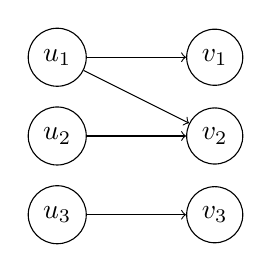
\begin{tikzpicture}[scale=1]
        % Define nodes for U and V
        \node at (0, 1) (u1) [circle, draw] {\( u_1 \)};
        \node at (0, 0) (u2) [circle, draw] {\( u_2 \)};
        \node at (0, -1) (u3) [circle, draw] {\( u_3 \)};
        
        \node at (2, 1) (v1) [circle, draw] {\( v_1 \)};
        \node at (2, 0) (v2) [circle, draw] {\( v_2 \)};
        \node at (2, -1) (v3) [circle, draw] {\( v_3 \)};
        
        % Draw edges
        \draw[->] (u1) -- (v1);
        \draw[->] (u1) -- (v2);
        \draw[->] (u2) -- (v2);
        \draw[->] (u3) -- (v3);
    \end{tikzpicture}
    \caption{Directed Bipartite Graph}
    \label{fig:bipartite-graph}
\end{figure}

To convert the bipartite graph into a flow network:

\begin{enumerate}
    \item \textbf{Introduce a source \( s \) and a sink \( t \)}.
    \item \textbf{Add edges from \( s \) to each vertex in \( U \)}: \( (s, u_1), (s, u_2), (s, u_3) \).
    \item \textbf{Add edges from each vertex in \( V \) to \( t \)}: \( (v_1, t), (v_2, t), (v_3, t) \).
    \item \textbf{Add edges between vertices in \( U \) and \( V \)} as per the original bipartite graph: \( (u_1, v_1), (u_1, v_2), (u_2, v_2), (u_3, v_3) \).
\end{enumerate}

The resulting flow network is shown in Figure~\ref{fig:flow-network}:

\begin{figure}[h]
    \centering
    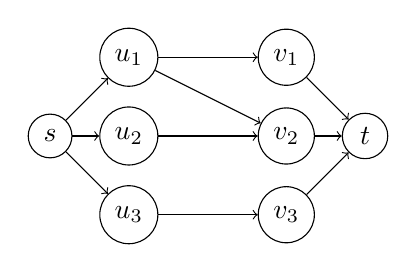
\begin{tikzpicture}[scale=1]
        % Left side vertices
        \node at (0, 1) (L1) [circle, draw] {\( u_1 \)};
        \node at (0, 0) (L2) [circle, draw] {\( u_2 \)};
        \node at (0, -1) (L3) [circle, draw] {\( u_3 \)};
        
        % Right side vertices
        \node at (2, 1) (R1) [circle, draw] {\( v_1 \)};
        \node at (2, 0) (R2) [circle, draw] {\( v_2 \)};
        \node at (2, -1) (R3) [circle, draw] {\( v_3 \)};
        
        % Source and sink
        \node at (-1, 0) (S) [circle, draw] {\( s \)};
        \node at (3, 0) (T) [circle, draw] {\( t \)};
        
        % Edges
        \draw[->] (S) -- (L1);
        \draw[->] (S) -- (L2);
        \draw[->] (S) -- (L3);
        \draw[->] (R1) -- (T);
        \draw[->] (R2) -- (T);
        \draw[->] (R3) -- (T);
        \draw[->] (L1) -- (R1);
        \draw[->] (L1) -- (R2);
        \draw[->] (L2) -- (R2);
        \draw[->] (L3) -- (R3);
    \end{tikzpicture}
    \caption{Flow Network Representation of Bipartite Graph}
    \label{fig:flow-network}
\end{figure}

Once the flow network is constructed, we can apply a maximum flow algorithm to find the maximum matching. The resulting maximum matching is:

\[
\text{Maximum Matching: } \{(u_1, v_1), (u_2, v_2), (u_3, v_3)\}.
\]

\noindent This is illustrated in the final Figure~\ref{fig:maximum-matching} below:

\begin{figure}[h]
    \centering
    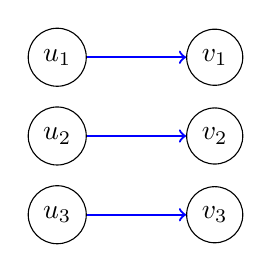
\begin{tikzpicture}[scale=1]
        % Left side vertices
        \node at (0, 1) (L1) [circle, draw] {\( u_1 \)};
        \node at (0, 0) (L2) [circle, draw] {\( u_2 \)};
        \node at (0, -1) (L3) [circle, draw] {\( u_3 \)};
        
        % Right side vertices
        \node at (2, 1) (R1) [circle, draw] {\( v_1 \)};
        \node at (2, 0) (R2) [circle, draw] {\( v_2 \)};
        \node at (2, -1) (R3) [circle, draw] {\( v_3 \)};
        
        % Draw matching edges
        \draw[thick, ->, blue] (L1) -- (R1);
        \draw[thick, ->, blue] (L2) -- (R2);
        \draw[thick, ->, blue] (L3) -- (R3);
    \end{tikzpicture}
    \caption{Maximum Matching in Bipartite Graph}
    \label{fig:maximum-matching}
\end{figure}
